\documentclass[10pt,conference]{IEEEtran}
\usepackage{cite}
\usepackage{amsmath,amssymb,amsfonts}
\usepackage{algorithm}
\usepackage{algorithmic}
\makeatletter
\newcommand{\algrule}[1][.2pt]{\par\vskip.5\baselineskip\hrule height #1\par\vskip.5\baselineskip}
\makeatother
\newcommand{\worklist}{\textit{worklist}\xspace}

\usepackage{graphicx}

\usepackage{textcomp}
\usepackage{xspace}
\usepackage{booktabs}



\usepackage[table]{xcolor}
\usepackage{paralist}
\usepackage{url}

\usepackage{boxedminipage}
\usepackage{enumitem}
\usepackage{graphicx}  
\graphicspath{
	{figures/}
}
\DeclareGraphicsExtensions{.pdf,.jpeg,.png}


% Complex \xxx for making notes of things to do.  Use \xxx{...} for general
% notes, and \xxx[who]{...} if you want to blame someone in particular.
% Puts text in brackets and in bold font, and normally adds a marginpar
% with the text ``xxx'' so that it is easy to find.  On the other hand, if
% the comment is in a minipage, figure, or caption, the xxx goes in the text,
% because marginpars are not possible in these situations.
{\makeatletter
 \gdef\xxxmark{%
   \expandafter\ifx\csname @mpargs\endcsname\relax % in minipage?
     \expandafter\ifx\csname @captype\endcsname\relax % in figure/caption?
       \marginpar{\textcolor{red}{xxx~}}% not in a caption or minipage, can use marginpar
     \else
       \textcolor{red}{xxx~}% notice trailing space
     \fi
   \else
     \textcolor{red}{xxx~}% notice trailing space
   \fi}
 \gdef\xxx{\@ifnextchar[\xxx@lab\xxx@nolab}
 \long\gdef\xxx@lab[#1]#2{{\bf [\xxxmark \textcolor{red}{#2} ---{\sc #1}]}}
 \long\gdef\xxx@nolab#1{{\bf [\xxxmark \textcolor{red}{#1}]}}
 % This turns them off:
% \long\gdef\xxx@lab[#1]#2{}\long\gdef\xxx@nolab#1{}%
}

% Double Blind Commands
\makeatletter
\newif\if@doubleblind
\@doubleblindtrue %use \@doubleblindfalse on final version

%Supporting On-line Material
\if@doubleblind%
\newcommand{\site}{(blinded URL)}
\else
\newcommand{\site}{\url{http://www.jonbell.net/software/pradet/}}
\fi

% Acknowledgment
\if@doubleblind%
\newcommand{\acknowledgment}{ }
\else
\newcommand{\acknowledgment}{
\section{Acknowledgment}
The authors would like to thank ...
}
\fi



\newcommand{\abc}{\textsf{ABC}\xspace}
\title{ABC: Action-Based Test Carving}

\if@doubleblind%
\author{Undisclosed Authors}
\else
\author{\IEEEauthorblockN{Alessio Gambi}
\IEEEauthorblockA{\textit{University of Passau} \\
%\textit{name of organization (of Aff.)}\\
Passau, Germany \\
alessio.gambi@uni-passau.de}%
}
\fi

\begin{document}

\maketitle

\begin{abstract}
\end{abstract}

\section{Intro and motivation}
Importance of tests, classes of tests and their pro/cons.
In this paper we focus on system and unit tests, specifically in their use for regression.

System tests are wide scoped, but "real" (~\cite{exysts}).
However, they take long time to complete because they need to setup/deploy the real system, and interact with it.
A common setup is the one to start the SUT and one or more "clients" which interacts with it.
System tests can be automatically generated, for example, via fuzzying and random exploration, assuming a proper driver/infrastructure is available.
For example, this is commonly the case for GUI (Exysts),  Web Application (with crawlers and Selenium) and Apps (Monkey).
%
In general, however, system tests for regression are setup manually: a designer/testers creates them to implement 
specific scenarios and test specific features (~\cite{TDD}-controlla nel libro).
%
For example, login into a system and buy a product, or rent a room. (Maybe better the latter so we keep around this for the test subject). 
%
This "ensures" to capture, during development, refactoring, etc. changes to the code which breaks funcitonalities. 

At the opposite spectrum, there's unit tests. Unit tests are focused, can be easily generated automatically (Evosutie and Randoop), and can achieve high coverage. However, (automatically) generated unit tests they might be "detached" from the reality, that is, they might implement executions which cannot be observed in real life (cite out paper at AST). Units test might turn out to  "waste" precious testing time.
Despite they might capture dangerous or problematic behavior of the SUT (e.g., an uncaught NPE), those problems might be only potential, and it might hard for developers to understand if the failing of a unit test is real or a false alarm.

In this work, we propose a novel approach for unit test generation based on the idea of carving unit tests out of system test executions. 
Elbaum et al~\cite{}\cite{}, which firstly present the idea of test carving, identify three types of approaches for carving:
state based carving, working on instances, aiming at recreating instances observed during system test execution based on heap state. 
Carving takes place on the object structure and identifies the relevant elements that define the state of an instance before and after a MUT to generate a test case. \xxx{check the paper again}.
Action based carving, which works by identifying and replaying only the method invocations that lead to a specific state of the CUT.
and Hybrid.
\xxx{Make sure it is clear they implemented and evaluated only 1}.
Elbaum and coahutors implemented and investigated only the first of these three approaches, and show \xxx{summarize the conclusion from the papers}.
In this work, instead we propose and to our knowledge implement, the first approach for test carving based on actions.
We show that, in line with the finding of Elbaum et al., the generated test cases implement the same behavior of system tests, are focused, \xxx{and faster} to execute than system tests (\xxx{add numbers here from the evaluation}).

\xxx{Summarize qualitatively the differences}
The two approaches, despite sharing the same underlying principle, requires different setup/infrastructures and produce different test cases.
\xxx{ provide an example code here of both}
%
The approach from Elabuam et all, requires an infrastucture for capturing and replaying the execution, which is based on serializing object instances.
\xxx{double check that the following is actually true !}
During the execution of system tests, instances are serialized after each method invocation and stored away. After carving, the differential unit tests
require the same infratructore for loading and restoring in the heap the object instances. This means that carved test cases cannot be execute outside the carving infrastructure. Additionally, carved test cases might be hard to read since the test cases hide the details of the objects being tests. 
As shown in Figure~\ref{fig:state-based-carving-example}, differential unit tests have a specific pattern: load a complex object from an XML file, 
invoke a method on this object, compare the resulting state to another XML file. Load and compare are opaque operations.

Notably, since this approach is based on object instance serialization and restore, it might (or not entirely) applicable for SUT which involve, non serializable objects (like file descriptors, network connections, connections to databased, etc), and SUT which have a distributed state. For example, it might be impossilble by means of pure statebased carving to recreate the state of an application which relies on a database (or even files) for persisting data.
Since de-serialization of the object instance, cannot recreate the inner state of the database (or file content).

At the contrary,  being based on action carving \abc does not suffer of those problems: once tests are carved, they do not require any specific infrastructure to be used. They in fact rely on the available testing infratructure (e.g. , JUnit and whatever test scaffolding the application used for system testing in the first place). This make carved tests ready to use. Second, carved tests are not opaque, but verbose (maybe they suffer of the opposite problem?).
That is, they explicitly replay the method calls to restore the original (or similar) application state (either this is distributed or local), and can be read.
%They follow the usual pattern, setup, execution \xxx{assertion}. 

In this paper, we do not focus on generating regression assertions, but during the carving we verify (using the same approach of Elbaum et al.) that the generate test cases lead to the same tests of the CUT before and after the test execution. Similarly, we obejseve that the return value of MUT produce the same results. Automatically generate regression assertions is a different problem than carving, hence we leave that for future work.

\paragraph{Contribution}
A novel approach to unit test case generation based via action-based test carving
An evalaution of this approach against test subjects which use Files and Databases to operate and shows that carved tests
implements the same beahviors of system tests, and enable optimizations of regression, which entails reducing the test execution time by X and, in average, reduce the amount of tests to execute up to Y.


\begin{figure*}[h!]
\centering
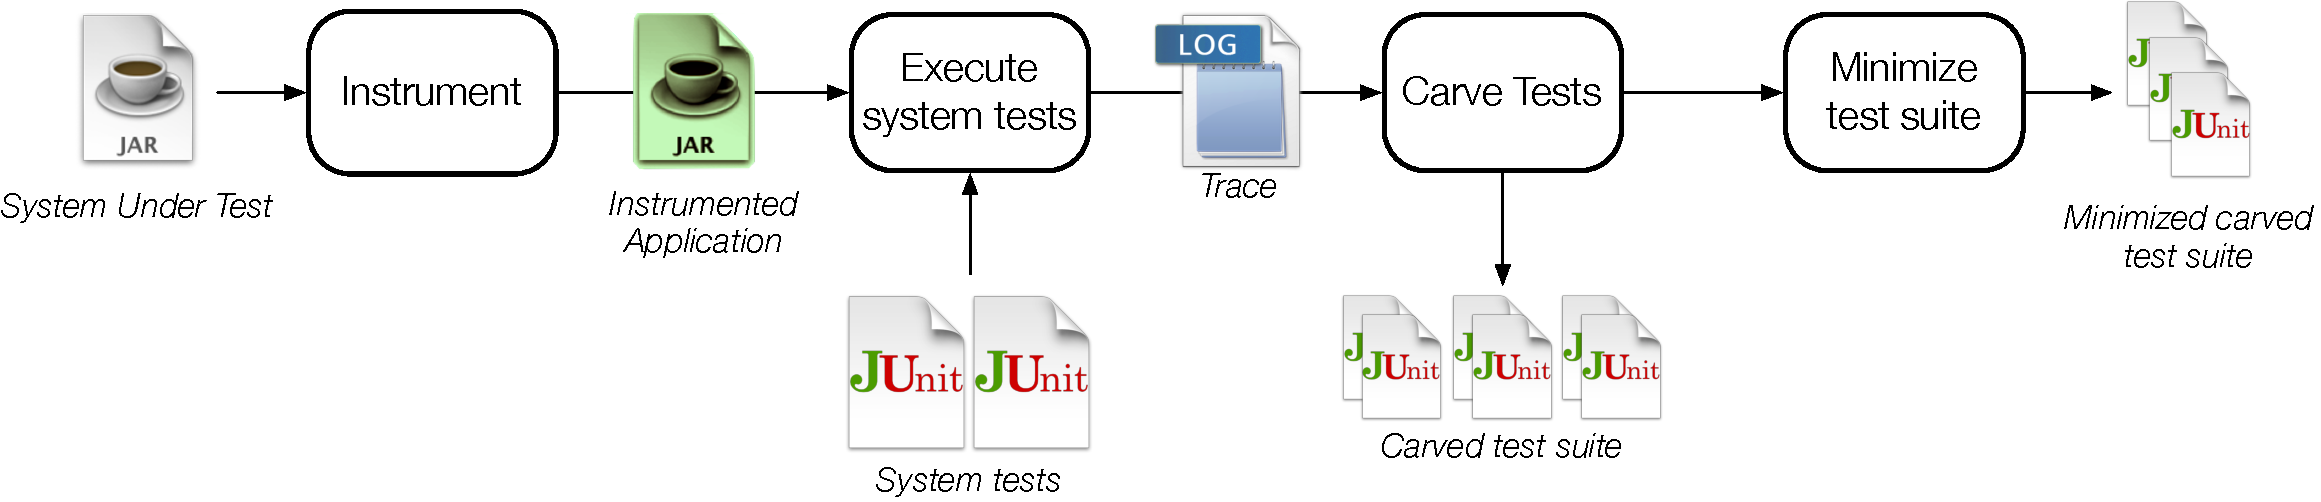
\includegraphics[width=\textwidth]{overview}
\caption{Overview of the \abc approach: \abc \emph{instruments} the application under test to inject tracing code; next, it \emph{executes the system tests} using the instrumented version of the application to generate a trace file and a copy of the instances processed during the execution; 
then, it \emph{carves} a set of shorter executions and \emph{validates} that those stress the units of code like systems tests
do. Finally, \abc \emph{reduces} the size of the carved test suite using delta debugging, before \emph{generating} the actual source code which implements them.
\xxx{Add delta debugging again}
}
\label{fig:overview}
\end{figure*}

\section{\abc Overview}
\xxx{A nicer intro better. Remark the meaning of action-based carving, which then clarify why we need data from dynamic executions of system tests to carve the tests.}

\abc implements action-based carving in four steps: instrumentation, tracing of system test execution, test carving, and test suite minimization. \xxx{what about delta debugging?} 

\paragraph{Instrumentation}
We instrument the application under test to inject code which traces the execution.
%
In particular, for each method invocation we trace the method being invoked, the owner of that method invocation unless the method is static, and the return value of the method invocation unless the method is void.
The method invocation owner is the object instance upon which the method is invoked.

Informations about method signature and method owner are taken \emph{before} the method is executed, while information about its return type are taken \emph{after} the execution.
%
We do so to avoid losing method ownership informations in case the control flow of the application is abruptly interrupted during the execution of a method, either because an exception is  thrown  or because the application terminates by invoking \texttt{System.exit}.
%, which prevents us to collect observereturn values and more importnatly ownership informations otherwise).

Instrumenting \emph{only} method calls is not enough to build a sufficiently complete trace of execution, that is, a trace which allows to rebuild the original execution of the application before carving int. 
Important informations, including assignments and access to fields, store and access to array elements, which are relevant to rebuild the data dependencies among method executions, would be missing from the trace of execution if we would track exclusively method calls.

To consider those information during the execution, we trace them as \emph{artificial} method invocations. 
For example, a statement like \texttt{A.f = v} is interpreted as an artificial method call to a static method 
\texttt{setField(String fieldName, Object fieldValue)} of an \xxx{ephemeral/fake} class \texttt{abc.Class}.
Similarly, a statement like \texttt{v = a[0]} is interpreted as an artificial method call \texttt{elementAt(int position)} of the array \texttt{a}.
%
Adopting this approach enables us to keep all the required information for test carving around and treat all \xxx{operations/statement} in the application in a standard and uniform way during carving.

Additionally, \emph{after} each method invocation we serialize the state of the return value and the state of the method invocation owner to files. Differently than the informations about method calls, which are mandatory for carving the test cases, such serialized state of the objects are optional and we use them to cross-check the correctness of our carved test cases.

In our prototypical implementation, we rely on Soot~\cite{} for instrumenting the application because the framework is rather intuitive, well supported, and we have previous experience with it; however, using Soot is by no means necessary to implement action-based test carving. As long as it can generate a complete trace of execution, any instrumentation technology can be used for this purpose. We rely on XStream~\cite{} to serialize object states into XML Files and persist the on disk because XStream is the de-facto library for object serialization in Java and the same library was used in the original work by Elbaum and co-authors to implement state-based carving.

\paragraph{System test execution and tracing}
We run the system tests using the instrumented code of the application under test to produce the execution trace and the dump of all the object instances processed during the execution. As common practice, before each system test we ensure the environment is not polluted and then we execute each system test in an isolate JVM, an execution mode supported by state of practice test execution frameworks~\cite{surefire-fork-isolate}. Additionally, we reduce this way the possibility of causing manifest test dependencies, flaky tests, and other problems related to polluted states which invalidated our analyses~\cite{Glicoric-or-Giory, Gambi,Bell,Ernt-DTD}.

\paragraph{Test Carving} 
Action-based test carving develops by identifying the method to carve and building a backward
slice which transitively includes all the method calls which potentially have an effect on the owner
of the method to carve and its parameters.
\abc does so by elaborating on three data structures that we derive from the trace of system test executions:
an execution flow graph, which captures the time-dependencies between method calls;
a data-dependency graph, which captures dependencies on data such as parameters, method owner, and return values;
and, a call-graph, which captures the structural dependencies of method calls and their nesting.

Action-based test carving not only carves the preconditions of the method under tests, but it also considers interactions with the external environment which might have an effect on the behavior of system under tests. Example of such interactions are accesses to the file system, databases, or remote services. Accessing the environment is typical done by means of specific interfaces, libraries and APIS. For instance, \texttt{java.util.Scanner} receives user inputs from the command line, classes inside the \texttt{java.io} and \texttt{java.nio} packages wrap calls to the underlying file system, and classes under the \texttt{java.sql} package enable database interactions. Since the list of the external interfaces is largely application specific, \abc enables developers to configure which external interface to consider and to specify additional external interfaces.
\abc includes interactions which potentially affect the behavior of the system under test by conservatively carving the calls to those  external interfaces which precede the call to the method to carve, thus ensuring that any precondition that tests have on the environment are met. Notably, this is impossible to achieve via standard state-based test carving, which controls only
the internal state of the application.

\paragraph{Test Validation}
\abc implements an additional validation step to check the validity of the carved tests. 
%
Some of the carved tests do not \emph{directly} invoke the method under carving; in this case,
despite the execution of those tests ``at some point'' produces the expected results, that is, the state of the class under test is the same observed during the execution of system tests, \abc report them as invalid and discard them.
%
The reason behind this choice is the observability of the results: Since the invocations 
 of the methods under test are not directly visible in the code of carve tests, there's no straightforward way
for developers to assert the behavior of the unit.

Other carved tests, because of improper definition of external interfaces or corner cases in the implementations of the application under test which \abc prototype does not handle, simply do not produce the expected result. 
We identify those tests by relying on the serialized object values that we collected during system test execution. From the XML dump of the serialized objects, \abc creates a set of test of basic assertions on the state of the unit under test after the methods to carve are invoked as well as on the return values they produce.
Those assertions, used in conjunction with typical implicit test assertions~\cite{randoop}, like uncaught exceptions, let us identify
 tests which produce an unexpected result and report them to the developers. We remove the failing tests from the carved test suite.
Since the assertions based on XML serialized object have the same drawback of the assertions generated by Elbaum and co-authors,
we remove the from the code of the carved tests before generating the final carved test suite. This way we ensure the creation of realistic executions, but give developers the freedom to create and use their own assertions. The generation of effective regression test assertions is an central topic in the domain of automatic test case generation, and we leave it for future work.

\paragraph{Test Minimization - Delta Debugging}
Since \abc adopts a conservative approach to include method calls which might affect the state and the behavior of the application under test, the resulting carved tests might be longer than necessary, executing more expensive calls to external interfaces than necessary. 
For this reason, \abc minimizes the size of the test methods by identifying and removing method calls which do not change the state of the application or alter its behavior via a technique based on delta debugging~\cite{delta-debugging}. 

\abc starts from the method call before the method under test, and moves backwards to the beginning of the test case.
At each step, \abc removes one statement from the test and re-executes it. If the modified test does not fail despite one statement was removed, \abc concludes that the removed statement does not influence the unit under test and moves on to the next statement. 
Otherwise, \abc concludes that the removed statement is indeed necessary to correctly test the unit, and add it back to the test. 
To decide if the test passes or fails, \abc reuses the same assertions used to validate the carved tests.
%, that is, we compare the actual state of the unit under test and the return value of the method under test against the values observed during the original execution of the system tests.

%By removing unnecessary methods calls from the carved tests \abc reduces their size to a minimum.
%reducing the overhead incurrend in consevatively include all the calls which potentially affect the unit under test.
Delta debugging requires to repeat the execution of the carved tests multiple times, hence it becomes expensive as the size of the carved tests
increases. Consequently, a naive implementation of delta debugging which tests each and every statement in the carved tests in
isolation is impractical. On the one hand, executing tests in isolation is \emph{per-se} extremely expensive~\cite{jonbell:vmvm};
on the other hand, testing \emph{all} the statements of carved tests is not necessary. Only the calls which \abc included conservatively
shall be tested as the remaining method invocations can be proven to be necessary for the successful execution of the
carved tests even without executing them. Therefore, a general solution is to trace among the carved method invocations the ones which might affect
the unit under test, test if they are actually necessary, and then remove them and all their preconditions, that is the method invocations that
were in place, only to enable a correct execution of the removed method invocations. Unfortunately, this solution is made complex by the fact
that the same instructions might be needed to set the preconditions of multiple calls, hence simply removing them is not possible.

In this work, instead of implementing such a generic but rather complex solution, we approach delta debugging in a simplified, yet effective way
and instruct \abc to delta debug \emph{only} the method invocations which belong to the external interfaces.
The motivations behind this choice are that invocations to external interfaces, such as querying a
remote database, are generally slower compared to standard method invocations so removing them speeds up the execution of the
test cases, and that compared to the total number of statements which comprise the carved tests, calls to external interfaces are relatively few,
, hence testing only them drastically reduces the amount of re-execution of tests needed. 
%
%Additionally, as a second optimization of delta debugging, \abc does not execute carved tests in isolation, but all in the context of the same JVM
%
%many tests as possible in the
%
%Therefore, instead of checking each and every call, \abc focuses only on calls which are
%marked as external interfaces.
%; however, this incurs in a large overhead, which strongly reduces the practical applicability of \abc a
%This makes them possibly easier to read and faster to execute. 
%
%Once again, we remove from the carved test suite those test  which after minimization implement exactly the same behavior.
%

\xxx{Test Generation - TBD}
How do we approach generation, what we need to take into account, how do we do that.

The last step is the actual test generation where we take carved and minimized tests are produce executable java (JUnit) tests. We use open source library to generate the java code from our internal representation based on jimple/soot.



\bigskip

At the end of this process, the generated test suite implements the same behavior of the system tests used to create the traces; however, instead of doing so by means of few wide scoped system tests, it uses a multitude of focused unit tests. As we show in the evaluation this enables developers to leverage traditional regression testing optimizations, such as regression test selection~\cite{} and test suite reduction~\cite{}, which are hardly possible or not cost-effective when applied to system tests.
\xxx{Note that coverage based reduction reduced system tests from 10 to 1 for Employee, and from 19 to 3 for HotelMe!!!}

\section{Action-based Test Carving with \abc}
\abc implements action-based test carving by computing a backward slice of the methods under carve which \emph{conservatively} 
includes the methods invocations that might contribute to the state of the unit under test and that might affect the behavior of the method under carve. \abc includes in the slice not only the method calls which belong to the application under test
and \emph{directly} affect its state and behavior, but also includes the calls to the environment which might
\emph{indirectly} affect the state and behavior of the application.

Consequently, \abc implements action-based test carving in two steps:
	\emph{core carving}, in which \abc carves those methods which directly influence the unit and method under carve;
	and, \emph{carving of external interfaces}, in which \abc carves the methods which interacts with the environment and
	might indirectly influence the unit and method under carve;

Both steps are implemented by the same carving algorithm, with the main difference that, 
core carving is focused, involves relatively few dependencies, 
but is specific to each invocation of the methods under carve; 
carving of the external interfaces, at the contrary, is broad, 
involves many dependencies, but its results can be shared among
differented methods under carve. 
% Is this really necessary?
As consequence, the former carving step is faster than the second ---ten
 to hundred times faster according to our evaluation--- but does not enable
 the caching of partial results, which is instead possible while performing the latter carving step.

Action-based carving requires three data structures to be in place:
an execution flow graph, a data dependency graph, and a call graph.
%
% Formal definition
The \emph{execution flow graph} captures the temporal aspects of the execution as chain of method invocations.
Hence, it is a directed acyclic graph, whose nodes represent method invocations and each method invocation is connected to the method invocation which strictly follows it in the execution.

The \emph{data dependency graph} captures the dependencies between method invocations through data, via method ownership, parameter passing, or return values.
%
More formally, the data dependency graph contains three types of nodes:
	\emph{method invocation} nodes which represent invocations of methods;
	\emph{object instance} nodes which represent references to non-primitive objects;
	and, \emph{value} node nodes which represent primitive types an un-mutable entities like \texttt{null}.
The data dependency graph constrains three types of directed edges:
	\emph{ownership} edges which connect non-primitive object instances to the method invocations invoked upon them;
	\emph{parameter} edges which connect object instances and values to the method invocations which require them as parameters;
	and, \emph{return value} edges which connect method invocations to the object instances or values which they return. 

The \emph{call graph} captures the caller-callee dependencies between method invocations, hence their nesting.
More formally, the call graph is a tree rooted in the \texttt{main} method, whose nodes are method invocations connected by means of directed \emph{invocations} edges. A method m1 calling a second method m2 is represented in the call graph by mean of a directed edge from invocation node m1 to invocation node m2.

% Core carving
\subsection{The Action-based Carving Algorithm}
Action-based carving starts by locating the invocations of
the methods under carve  in the graphs, and for each of them applies
Algorithm~\ref{alg:carving} for computing their carved execution.
%
Once the carving is over, \abc assembles the carved tests by merging
the carve obtained for the application invocations with the carves obtained for
the external interface invocations.

\begin{algorithm}
\caption{Action-based carving of method invocation $m_X$}\label{alg:carving}
\begin{algorithmic}
\REQUIRE$ $
\STATE$\text{Execution flow graph } \mathcal{E}$
\STATE$\text{Data dependency graph } \mathcal{D}$
\STATE$\text{Call graph } \mathcal{C}$%
\end{algorithmic}
%\\\hrulefill
%\makeatletter
%\setcounter{ALC@line}{0}
%\makeatother
%\xxx{Even if this is not the actual implementation which can compute the cartesian product of calls, our evaluation is done according to this algorithm}
\begin{algorithmic}[1]
\algrule
\STATE $worklist \leftarrow \{ m_X \}$
\STATE $slice \leftarrow \{\emptyset\}$
\WHILE{$ worklist \neq \emptyset$}
\STATE $m \leftarrow worklist.\text{poll}()$
	\IF{$m \in slice$}
		\STATE $\textbf{continue}$
	\ENDIF
	% Compute direct method dependencies of m
	\STATE $s_m \leftarrow \mathcal{E}.\text{before}(m) \cap \mathcal{D}.\text{reachable}(m)$
	\STATE $worklist.\text{enqueue}(s_m)$
	
	\STATE $slice.\text{append}(m)$
	
	% Compute data dependencies
	\FOR{$o \in \mathcal{D}.\text{dataDeps}(s_m)$}
		\STATE $worklist.\text{enqueue}(\mathcal{D}.\text{methodReturning}(o, s_m))$
	\ENDFOR 
\ENDWHILE
\algrule
\STATE $subsumed \leftarrow \mathcal{C}.\text{getSubsumedCall}( slice )$
\IF{$m_X \in subsumed$}
	\RETURN$NOT\_A\_VALID\_TEST$
\ELSE
	\IF{$\text{unsafe}(slice,subsumed)$}
		\RETURN$\text{recovery}(slice, subsumed)$
	\ELSE
		\RETURN$slice \setminus subsumed$
	\ENDIF
\ENDIF


\end{algorithmic}
\end{algorithm}

Algorithm~\ref{alg:carving} works by elaborating a \worklist which contains the method invocations yet to be carved,
and a \emph{slice}, which accumulates the method invocations carved so far.
At the beginning, \abc initializes the \worklist with the method under carve, $m_X$, and an empty slice.
From that point on, the algorithm iterates until the \worklist becomes empty.

At each iteration, a new method to carve is taken from the \worklist and processed unless the methods
belongs already to the slice, in which case the algorithm continues with the next element.
%
Given a method invocation to carve, $m$, \abc computes the backward slice, $S_m$ for it by intersecting the set of
method invocations which happened before $m$ according to the execution graph $\mathcal{E}$ with
the method invocations reachable via data dependencies from $m$ in the data dependency graph $\mathcal{D}$~(line 8). 
Method calls reachable via data dependencies include all the methods calls invoked upon
the owner of method invocation $m$, such \abc can recreate the proper state of that object in the carved test.
%
Next, \abc enqueues the backward slice $s_m$ in the \worklist to transitively carve all the methods therein, and
updates the slice by appending $m$ to it.

Then, \abc computes also the set of object instances which participate in $s_m$ and which must be included in the carved
test by means of the data dependency graph $\mathcal{D}$~(line 11). For each of these object instances, \abc selects a
suitable method which returns them to be included in the carve tests, and enqueues it in the \worklist.

Object instances are always returned by their constructors; however, in practice, other methods might return them and the choice
of which method invocations to use to return these instances in the carved tests is non trivial.
% This makes action-based test carving a challenging problem to solve.
%to return the instances in the carved tests. This makes action-based test carving a challenging problem to solve.
%
Some classes declare only private constructors and their instances can only be obtained via static methods. 
This is, for instance, the case of classes which adopt the singleton or the object factory design patterns~\cite{designpatterns}.
%
In this case, the carved tests cannot directly instantiate the objects, and \abc must select the proper methods
which can return the required instances. This also includes correctly setting up the singletons and object factories which
provide them.
%
In other cases, the required object instances are stored as fields inside other objects instances, which expose them
via getter methods or as public fields. In this case, \abc must decide which strategy is more convenient to adopt
to carve them: either, directly invoking the constructors and explicitly setting the object instances, or carving the
methods of their container objects, and getting the required object instances via getter methods.
%
As basic strategy, \abc favors the former strategy, so in the carved tests all the steps which leas to correctly set up
the test preconditions are clearly visible. However, this is not always possible since object instantiation and setup must
not conflict with the other method invocations carved so far. In particular, \abc must ensure that in the context of a carved
test execution, method calls are invoked exactly the right amount of time, which is challenging since carve tests might mix 
and match method invocations from different locations.

To address this challenge, \abc collects for each object instance all the methods which return it, 
and selects among them the non-private method invocation which is closest to the method invocations currently
under carve according to the call graph $\mathcal{C}$. Consequently, \abc enqueues the selected method calls into
the \worklist to carved them as well (line 12).

Note that \abc does not track or follow the data flow of primitive values, hence it does not include them to compute the backward slice.
Carving of primitive values is not needed since primitives type do not require any setup, are immutable, and are passed by value. 
%This greatly simplifies the carving process and
%enables \abc to exclude from the carved tests many method calls. 

Eventually, the algorithm reaches a point where no more method invocations need to be carved, 
and the generation of the carved test begins (line 15-24).
%For instance, this happens when the method under carve does not receive objects instances as parameters.
Test generation consists in computing and removing the \emph{subsumed} method invocations in the slice as
well as ensuring that carved tests meet basic properties.

A method invocation subsumes another one, if the latter is transitively invoked in the scope of the former;
that is, if the execution of a method $m_1$ either directly or indirectly results in the invocation of method $m_2$, 
then $m_2$ is subsumed by $m_1$.
%
If a slice contains method invocations which are subsumed, its execution results in invoking those methods multiple times.
This, in turns, might affect the behavior of the unit under test and invalidates the carved tests. 
% Hence \abc removes sub them.
\abc relies on the call graph $\mathcal{C}$ to compute the set of method calls subsumed in a slice (line 15).

Removing subsumed method invocations from the slice results in one of the following three situations:
First, the subsumed methods invocations contain the original method under carve, $m_x$. 
Removing the subsumed calls ends up removing $m_x$, which violates the very basic observability property of unit tests.
\abc reports the error and skip the generation of this test~(line 17).

Second, the subsumed methods invocations contain calls to constructors which instantiate objects used later in the test;
at the same time, subsumed methods invocations do not contain all the method invocations upon those instances. 
Therefore, removing them ends up removing the calls to the constructors, but leaves the calls to the objects which is un-safe
since the objects are not initialized~(line 19). \abc tries to recover from this situation by replacing
the unsafe calls with replacements calls which subsume them; this way, it can ensure that all and only the necessary calls
 are made safely upon those object instances. If a recovery is not possible or fails, \abc reports the error and
 skip the generation of  this test~(line 20).

Finally, if the subsumed method invocations are safe to remove, \abc returns the reduced slice as output~(line 22).
At this point, the action-based carving algorithm terminates by ensuring that either the generated slice contains all the relevant
method invocations to ensure a correct invocation of the method under carve $m_x$ as well as all the methods which set
 its preconditions, or no test is generated.


%% Carving of EI and caching
%Carving of External interfaces (conservative): Users list the external interfaces upon which the SUT depends. Common interfaces include java.io.Files, java.nio.Paths which act as interface/api to the underlying File System, classed under java.sql which acts as interface to Sql databases, and java.util.Scanner, which act as interface to the user (via the Console/command line). We carve invocations on those external interfaces by recursively carving all the invocations to them which happens before MUT and which are NOT yet included in the CORE carving, to avoid calling external interfaces multiple times. For carving, we proceed similarly to Core carving \xxx{Double check the algorithm if we still consider combination of inputs}.

%\subsection{Including test setup methods}
%\xxx{This is an optimization to improve efficiency, however, it might not be safe: we need to guarantee that test setup methods do not interfere. Additionally, if we say we have this, WHY do not we use it anywhere? Plus, we need to show the effect on the results otherwise its just blabbing. Do this only if you have time left}
% Including test setup methods - This is to avoid polluting the environment, we rely on user to define those.
%Including test setup methods (conservative): We do not instrument nor carve test setup methods, like the one commonly executed inside @Before.
%The motivation here is that those methods configure the test environment for the system tests, i.e., they do not belong to the application logic,
%but rather to system tests logic. Nevertheless, carving tests (might) require those methods to be in place. For example, a typical setup method drop and recreate the mysql database. This ensures that system tests start from a known state of the database. Since tests carved from the system tests rely on the same assumptions, we need to include and replicate the same setup before executing them. Again we adopt the conservative approach of including all the required setup calls to generate carving tests. This has the benefit to ensure that the right preconditions are in place, but has the drawback to increase the execution overhead of the carved test. Imagine the case a carved test performs a basic check on an input, i.e., the input shall be greater than 0. If this test was carve out of a system test which requires a databased filled with test data, our conservative approach will recreate the databased also for the carved test, unnecessarily. Because of this, we will proceed by minimizing the test cases and removing all the unnecessary method invocations from the carved test.

% Similarity check and duplicate removals

% Mocking input values and system.exit ?

% Test Generation and test code generation

% Validation

\section{Evaluation}

\textbf{Goal of the evaluation} 

Show the usefulness of test carving by means of showing that 
carved tests stress the SUT in the same way systems test do, but at the unit level. 
That is we do not lose testing power/miss behaviors by using carved tests.
%
We illustrate this by showing how code coverage achieved by system and carved tests is the same.

\paragraph{Test case selection reduction}
Carve tests are more focused than system tests, hence, in a regression setting we do not necessarily need 
to execute all of them. This is not true in general for system tests which, by involving the entire system, end up in using (hence depending on)
all the system classes (or at least a great deal of it).
%
We illustrate this by modifying the system under test (using bogus, non-logic-modifing modificaitons) and counting how many system and carved
tests are executed after each modification. In particular, we show that modification of few classes already caused all system tests to be triggered,
while only a relevant subset of carved tests are re-executed.

\paragraph{Test suite reduction}
Carved tests are much more than system test, many of the carved test stress the same code of the application, although under different execution conditions. Therefore, they achieve the same coverage, and can be easily eliminated if one is interested in achiving a regression test suite optimized towards coverage.
%
We illustrate this by performing a test suite reductions on carved tests and showing that we can remove many (up to 80\%) of the carved tests, compared to removing barely 10\% of system tests.

Additionally, even reduced test suite, show benefits for RTS.

\paragraph{Overhead of Delta Debugging}.
Delta debugging -> this one becomes part of the evaluation. Since we adopt a conservative approach to include all the calls which might be state chaging,
we are interesting to investigate if this is "a bad thing". How many of those actions are superfluous and can be safely removed?
This also gives us a hint on if/how it would be beneficial to use delta debugging to minimize the carved tests cases.

For doing so, we implemente a delta debugging appraoch to remove and test each action, and compare the results on execution time, coverage and regression test selection of original and minimized test to see.
	generate validation instruction based on XML serialized state. We do not literally compare the serialized state, because some objects cannot be serialized in a meaningful way (i.e., open data base connections, file descriptors, streams) and some objects are parameters of the tests and are injected as dependencies during testing. For example, temporary working dir, date objects relative to current date, and other data that are generated randomly at the beginning of each test (and never changed during the execution?). 
	
Note: our apporach to delta debugging is naive, we simply try out all the instructions, however, we can also optimize the process by considering which method calls we included inside the tests because their were deemed necessary versus calls that we included because we'have been conservative. Additionally, we do not have to necessarily try out all the statement that we included for being conservative. Imagine we include method X, to call it, we needed to include all its preconditions. At this point, the moment we remove X, we can automatically remove all its preconditions - unless those are shared among other methods. This saves time, since we do not need to delta debug also the instructions needed to setup a given (and already proven useless) method X.
	
	\xxx{Give examples here on Employee and HotelReservation ? this means we need to introduce them as motivating scenarios?}
	
	Otherwise, we cannot remove dependencies correctly. \xxx{This requires an example}.
	We compare both the return value of the MUT if any, and the state of CUT.
	
	Starting from the instruction before MUT and going backwards, we remove one instruction, repeat the test execution, and check that the test passes. That is, no unhandled exceptions and no failed assertions.

	We assume a reset environment function, i.e., wipe out the database, is provided by the user to avoid polluting, and invalidating the result of delta debugging. Note that the carved tests instead do not require this, and are correct by design.
	
	\xxx{How much do we save in terms of instructions? and execution time?}

This is simple but effective solutions, however, it incurrs in a huge performance overhead because each carved test must be re-executed a number of times equals to the amount of instructions it contains. Optimization based on static analysis and data-flow analysis might be used here to identify cluster of invocations that belong together and possibly can be removed or left in the carved test all together. However, this is out of the scope of this paper and will be addressed in future work.
	\xxx{How much does it cost to run delta debugging?}

Benefits of Delta Debugging. Since delta debugging is expensive, we want to investigate/assess its cost/benefits. We do so by comparing execution time and number of instructions before and after minimization, as well as regression test selection.
%
Note that in this cases the evaluation is biased by the choice of the test subject, which do not involve external services (which might be slow and expensive to use), but only locally available resources.

\xxx{Maybe seel this thing of delta debugging as part of the evaluation to show that, because delta debugging does not remove many instructions, 
then the carved tests are already good, cannot be improved in that sense. Note that this accounts for the instructions not the method invocations executed !}

Overhead of carving, scalability of the approach. Longer execution of system tests generate larger traces, which requires to consider more and more invocations (since we conservatively include ALL the method calls to interested objects)

We are also interested in assessing the overhead of the overall approach to derive conclusions on its practical applicability.
For this, we measure and report execution and slow down factors of instrumentation, tracing, carving, test generation, and delta debugging.

\xxx{Carving time per method? per class?}
\xxx{Carving time vs Place in the trace/size of the trace/amount of system tests}
\xxx{Carving time vs type}
\xxx{Carving time vs number of arguments}
\xxx{Carving time vs Object to be carved}
\xxx{Carving time vs Type/System tests}

Overhead of Minimization ?
\xxx{size of test suites}
\xxx{size of test suites}


I suspect that delta debugging might shows benefits for those classes which do not involve or depend on external interfaces,
and are used frequently.
For example HotelView has barely no logic, but to test it there's a lot of setup that can be removed.
Really relevant?


\xxx{Carved tests are faster to execute than system tests.}
\xxx{Maybe we can show this per class under test: we need to execute only a subset of tests}
\xxx{With our test subjects, we cannot really shows this, since the time}

\subsection{Test Subjects}

Employee project.
Interactive command line utility to manage employee and salaries. It works by creating, reading, and deleting files.
\xxx{check if the same (or similar) to original carving work}
\xxx{Add stats?}

HotelReservation System project.
Interactive command line utility to handle an hotel reservation system. It uses mysql backend to manage the state of the applications.
\xxx{Add stats?}

\subsection{Experimental Settings}
System tests. The test subjects do not come with system tests, so I created them manually.
System tests work by resetting the state of the system before each test, mocking input commands, and cleaning up the state of the system
to avoid pollution~\cite{pollution}.
Additionally, system tests set up expectations on System.exit to avoid system and carved tests to abruptly halting the execution.

For the  Employee projects, I rely on temporary folders and predefined file contents.
For the HotelReservation, I rely on truncating the database and recreate it as expected (either empty, or with predefined content).

\xxx{How system tests are defined? Ideally I would like to create them by following a standard technique, in practice, I will motivate my choice
by saying I creating them to cover as much application state as possible, in a black box style.
That is, I consider "each" page of the application as state and navigate the application states by means of different input sequences.
The name should be coverage-transition? Check on the software testing class}

% Maybe a bit to verbose
To answer RQ1 and RQ2, I execute the system tests and measure the achieved coverage;
Next, I instrument the application,  repeat the execution of the same system tests to collect the trace, 
and from the trace carve the tests out. I generate carved tests and minimized carved tests using delta debugging.
Finally, I execute the carved and minimized carved tests to measure coverage, time to carve tests, 
time to generate tests, and time to minimize test via delta debugging.

To answer RQ3 I proceed as follow. 
Usefulness of Carve Tests:
I execute the Ekstazi tool~\cite{} on the original version of the code separately for system and carved tests.
Then, I randomly change a number of source files n (n={1, \ldots, N}, N is the total amount of application files (no tests, no Main)) in the project.
Next, I re-execute Ekstazi separately for ssytem and carved tests, but keeping the same modification , and collect information on how many system and carved tests where executed upon each modification.
Ekstazi will select only the tests which are needed to be re-execute to test the modification.
The modification is bogus, we do not modify for simplicity interfaces, but only implementation classes to avoid compilation problems.
We repeat the process for 20 times and for n from 1 to N (N is application classes)

\subsection{Results}

%\begin{table*}
%\centering
%\caption{Summary of Test Carving}
%\begin{tabular}{l l l l l l l l l}
%Project & System Tests &  Carved Tests & Class Coverage & Statement Coverage & Branch Coverage & time SYS &  time Carv &  time Carv MIN\\
%Employee & 7  & 87 &  100\% & 35\% & 14\%  & 0.045 & 0.081 & --\\
%Hotel Reservation & 5 & 145 & 100\% & 41 \% & 29\% & 0.615 & 7.78 & --\\
%\end{tabular}
%\end{table*}

\begin{table*}
\centering
\caption{Summary of Test Carving.}
\begin{tabular}{l l
			r r r
			r r r
			r r r
			r r r 
			r}
\toprule
\multicolumn{2}{c}{Project} & 
	\multicolumn{3}{c}{Tests (\#)} &
	\multicolumn{3}{c}{Execution Time (sec)} &
	\multicolumn{3}{c}{Stmt. Coverage (\%)} &
	\multicolumn{3}{c}{Branch Coverage (\%)} &
	\multicolumn{1}{c}{Trace Size (\#)} \\
	\cmidrule(rl){1-2}
	\cmidrule(rl){3-5}
	\cmidrule(rl){6-8}
	\cmidrule(rl){9-11}
	\cmidrule(rl){12-14}
	
	
	\multicolumn{1}{c}{name} & \multicolumn{1}{c}{feature} &
	\multicolumn{1}{c}{\textbf{S}} & \multicolumn{1}{c}{\textbf{C}} & \multicolumn{1}{c}{\textbf{M}} & 
	\multicolumn{1}{c}{\textbf{S}} & \multicolumn{1}{c}{\textbf{C}} & \multicolumn{1}{c}{\textbf{M}} & 
	\multicolumn{1}{c}{\textbf{S}} & \multicolumn{1}{c}{\textbf{C}} & \multicolumn{1}{c}{\textbf{M}} &
	\multicolumn{1}{c}{\textbf{S}} & \multicolumn{1}{c}{\textbf{C}} & \multicolumn{1}{c}{\textbf{M}} &
	 \\
\midrule
Employee & File system &
	11  & 454 & 9 & 
	5.1 & 2.1 & 0.2 & 
	73 & 73 & 73 &
	44 & 44 & 44 &
	5,470 \\
Hotel Reservation & SQL database & 
	17  & 976 & 46 & 
	12.5 & 91.4 & 4.3 & 
	82 & 82 & 82 &
	64 & 64 & 64 &
	35,820 \\

\bottomrule
\end{tabular} \\
\flushleft{The table reports an overview of the results achieved by \abc.
The \textbf{S} label identifies results for system tests, while \textbf{C} and \textbf{M} identify respectively the results for the carved and minimized test suites.
\xxx{Check if the achieved coverage is close to the maximum coverage that can be using only system tests!}
}
%\xxx{20 repetitions for the execution time}s
%	\multicolumn{1}{c}{Carving Overhead} & \multicolumn{1}{c}{Reduction} & \multicolumn{1}{c}{Delta Debugging}
%& 4,106 
%\xxx{Repeat the analysis and that the average execution time}
\end{table*}

\begin{figure*}[t]
\centering
\begin{minipage}[b]{.45\textwidth}
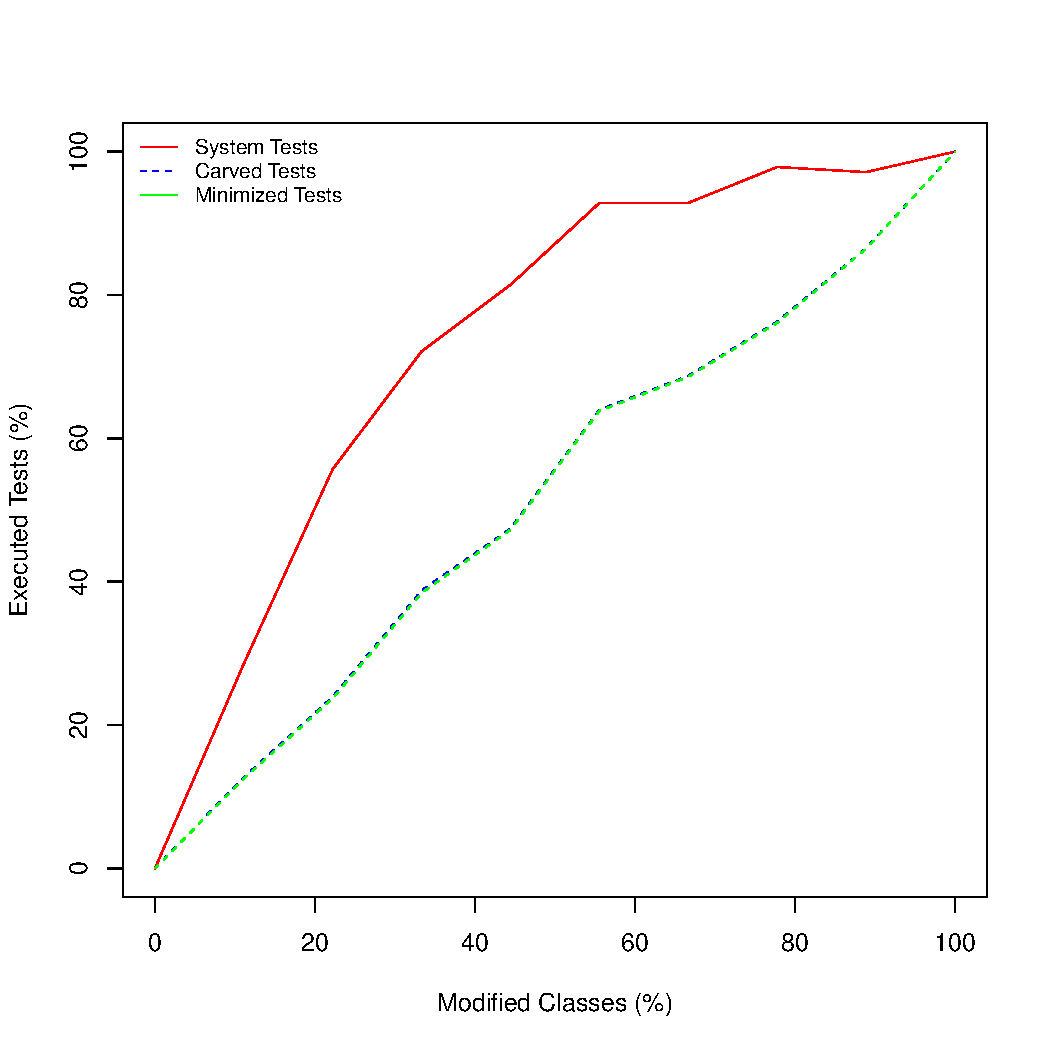
\includegraphics[width=\columnwidth]{figures/employee-rts-size}
\caption{Test Regression Selection - Employee}
\xxx{Make a Box Plot here instead. Lines connecting the average values, but boxes to show min/max ? Maybe consider splitting the plot in differen plots one for each approach, so it might be easy to compare?}
\end{minipage}\hfill
\begin{minipage}[b]{.45\textwidth}
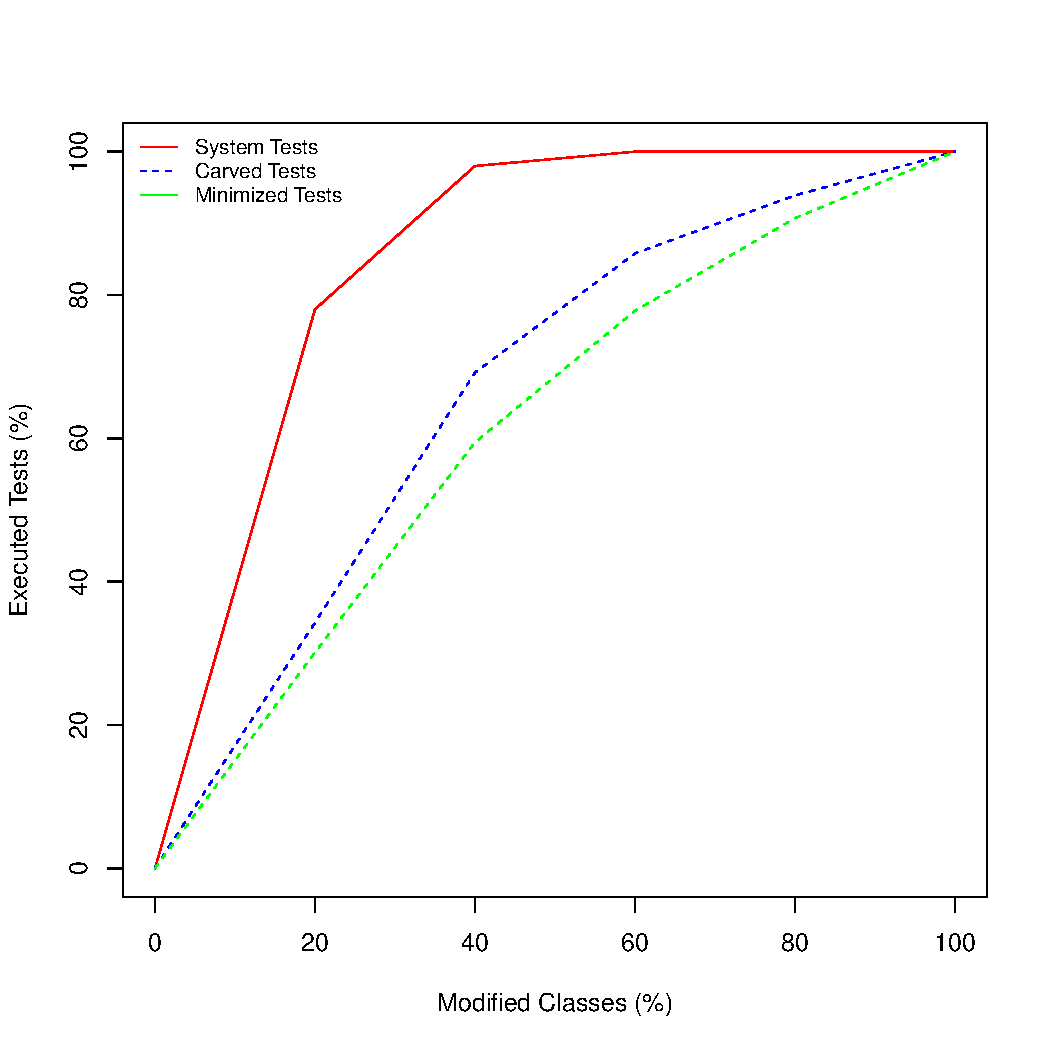
\includegraphics[width=\columnwidth]{figures/hotelme-rts-size}
\caption{Test Regression Selection - Hotel Reservation}
\end{minipage}
\end{figure*}


\begin{figure*}[t]
\centering
\begin{minipage}[b]{.45\textwidth}
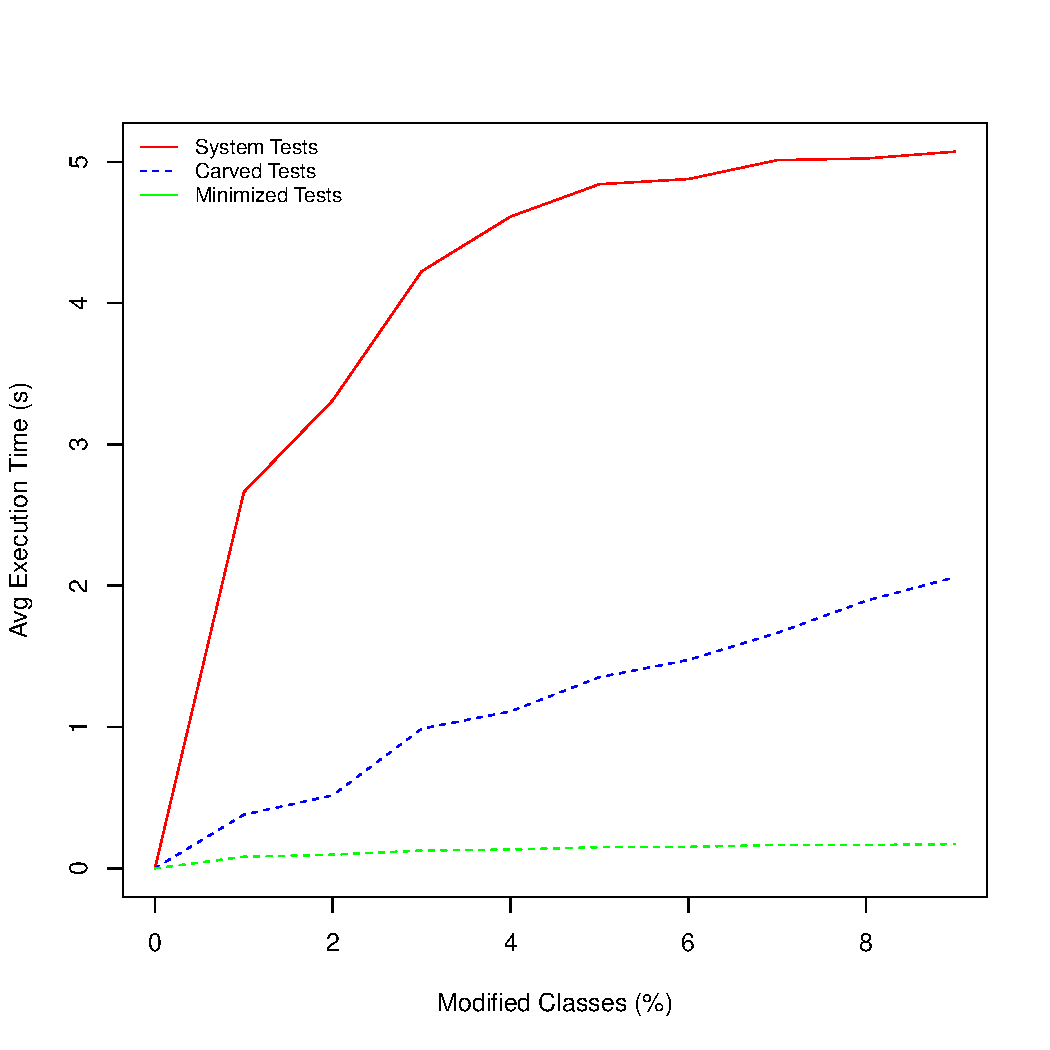
\includegraphics[width=\columnwidth]{figures/employee-rts-time}
\caption{Test Regression Selection - Execution time - Employee}
\xxx{Not sure this is relevant - update the system tests to last longer and explore more app behaviors}
\end{minipage}\hfill
\begin{minipage}[b]{.45\textwidth}
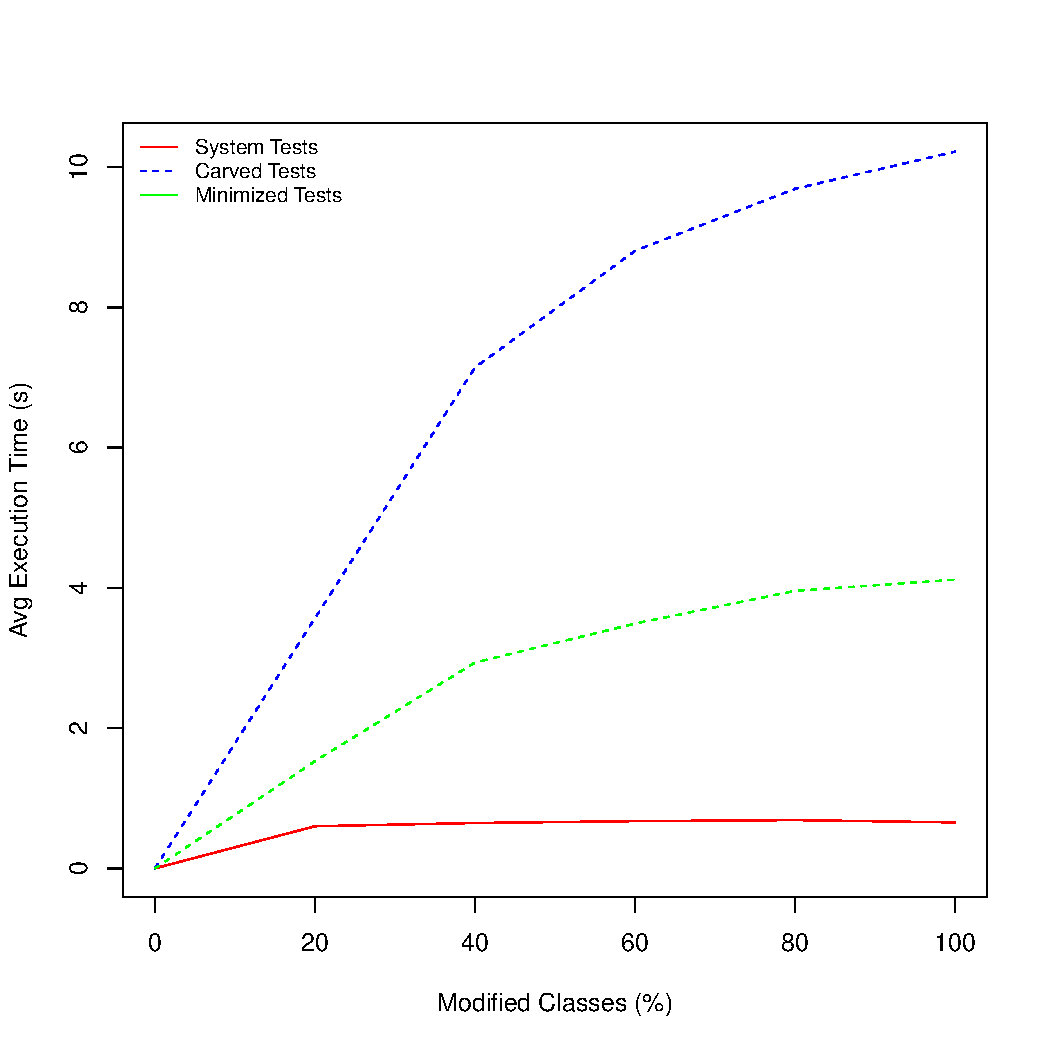
\includegraphics[width=\columnwidth]{figures/hotelme-rts-time}
\caption{Test Regression Selection  - Execution time -  Hotel Reservation}
\xxx{Not sure this is relevant - update the system tests to last longer and explore more app behaviors}
\end{minipage}
\end{figure*}

\subsection{Observation}
\xxx{For employee, Why the number of carved tests keep changing for hotel me?}
\xxx{For some }


\subsection{Discussion}
Coverage is the same

Execution time is larger for carved unit tests fro projects with simple setup.

We can generate tests for all the classes

Does minimization make sense?


Should I keep or not the test setup calls intact? Should I instead disassemble those as well ?!

Delta Debugging dominates the test generation time.
There's no difference in RST with and without minimized test cases.
For SOME REASON the minimized tests it takes more time to execute than the normal ones..
%
How many tests minimized? and how much?
%Employee: 87, 13 minimized (~14\%), those have an avg minimization of 95.55\%

% Is there a differnce in RTS.
Employee: there no difference in RTS, exactly the same tests are selected upon the same modifications.

\subsection{Limitations}
Action based carving need to "see" how object instances are created, otherwise might not be able to perform the carving because there's no way for the carver to reconstruct the object instance.

We observed this problem for example with test setup calls?

\subsection{Discussion}

Complex programs with GUI and WebApplications call for a hybrid approach: the hybrid approach provides (if possible) the parameters to the entry points of the application, for example, the servlet or the logic behind the GUI, which otherwise cannot observe the object creation thus replicate it.
With an hybrid approach, one might serialize the parameters of the calls and reload them to spin off the carving. E.g., one can define mocks that provide http requests, fill in with values objserved during the execution.

% Add biblio

\subsection{Conclusions and Future Work}


\abc is a young research, and the road to efficiently carve test cases is long and full of opportunities.
For the next future, we plan to address ...
%\section{Limitations and possible improvements}

\textbf{Non-carvable unit tests}
There are situations in which \abc cannot carve unit tests "at level-0/object interface". For example, \abc cannot carve methods which have "inner/outer" dependencies. That is, methods mX, which are called by outer methods mY, but at the same time requires inputs from the owner of mY. In this case, carving mX requires to include mY and all the methods called on mY owner, which eventually subsumes mX and therefor invalidate the basic property of (our) unit tests, which requires the CUT and the MUT to be directly visible/called in the test code. 

There might be different strategies to deal with this, but none necessarily general and applicable to all cases.
For example, we can break method dependencies: \abc might rely on developer provided information to break the dependency between mX and the owner of mY, such that it is not included in the carved test. This is for example the case of having a constant to be provided via a method by mY owner. In this case, "any" instance of that object would work the same. We might break the dependency by using an hybrid approach to provide a copy of the required value, under the assumption of not having side effects on the owner of mX. This for example is the case where the value is a primitive value or a string. 

A completely different strategy to test that specific method invocation consists in violating the basic property of level-0 test cases, and generate test cases which invoke the method subsuming mX but capturing and exposing the CUT and the result of the MUT, for example by smart checkpointing or mocking, or by directly injecting into the application code assertions to be invoked right after the target MUT. This, however, requires a smart infrastructure, similar to a debugger, to be in place during test execution to capture the precise moment the target MUT is invoked (simply imagine that MUT is invoked inside a for loop, and we are interested in generating a test case which check the 2 invocation of that method !). The development of such a smart testing infrastructure is part of our ongoing effort for carving test cases out system tests executions. 

Remarkably, the fact \abc cannot carve unit tests, might be also used to investigate the testability of an application. Infact, in many cases, failing to carve "inner/outer" test cases, is not always a problem with \abc but with the application itself, which simply has an hard-to test/bad design. Studying how \abc can identify \xxx{code smells} to assess the testability of an application is part of our on-going research effort.

\textbf{Missing observations}

\textbf{Missing observations due to Exceptional behaviors}

When an exception is thrown and not caught methods do not complete regularly, as a consequence, we do not trace their returns and the trace might be incomplete. The trace cannot be correctly parsed since we expect to observe a return from each method invocation.  Therefore, we might not correctly carve some tests.

\textbf{Missing observations due to partial instrumentation}
Difficulty to reconstruct objects which cannot be observed. Trace might not include the calls which generate an object instance, therefore a test which uses that cannot be carve. For example, tomcat provides httprequest object, we are interesting to carve the calls to our JSP/Servlets, plus we do not instrument (atm) Tomcat itself. So there's the need to get to the httpRequest object in the first place. This can be addressed by instrumenting tomcat (huge traces, huge overhead) or by extending \abc to implement an hybrid approach to test carving: the idea would be to use serialized versions of the objects for which we cannot observe setup and configuration (state-base carving), and then rely on action based carving to carve out the other tests. Carved objects might be then reconstructed using a search approach similar to the one proposed by Denaro et al~\cite{} or by Gligoric et al.~\cite{}. Integration with those approaches and extension of \abc are left for future work.

Implementation does not cover all the cases? Can be addressed by extending the instrumentation to cover them.
For example, we can trap exceptions and invoke artificial method calls. We might extend the scope of the instrumentation to capture object initialization. Those can be done without extending the approach but just the implementation. Alternatively, we can extend the approach to become hybrid.

\textbf{Scalability}
If we face long execution of system tests which generate huge traces traces of sheer size, \abc requires to consider many invocations inside its carved  tests. This is a consequence of conservatively include ALL the method calls to interested objects observed BEFORE the invocation of MUT.
This might raise scalability concerns, because the carving time becomes larger as the trace becomes larger.

To address scalability we employ several mechanisms:
we separately carve test cases for each system test, and we heavily rely on caching.
For example, in the context of the same system test, many objects share the same preconditions either because they depend on
the same input objects or because they require the same invocations to external interfaces. In those cases, instead of 
re-carving the same over and over, we provide the preconditions using the cache.

This however, has little effect for situations in which the preconditions do not exactly match. For example, if the same method is invoked in different
times, the later invocation of the same method include the same preconditions of the previous method calls, but also inculde all the method calls on the objects and external interfaces that happened between them. One strategy that can be employed in this case, which is similar to what Randoop does to build randomized sequences, is to carve preconditions incrementally. So instead of rebuilding the preconditions from scratch, we can rely on 
%
That is, by forcing the carving of methods according to the order of appearance of MUT, we can rely on caching partial setups.
\xxx{Maybe we can try this out if we have time before the submission?}

\textbf{Scalability - Too many test cases}
Another aspect related to scalability is the generation of many (too many) carve tests. On one side, this give developers the freedom to chose which carved test to select and expose the diversity of the behaviors stressed by the application, on the other side, many of the carved test cases are similar to one another.

We partially address this by filtering out test cases that are similar (at JIMPLE level) at the end of test carving, and to some extend during test case generation. However, we perform only basic checks, mostly syntactical, and those might not be as effective as smarter similarity metrics.
We also perform a test suite minimization based on coverage (and delta debugging?) This is effective to remove tests which do not contribute to coverage, but completely disergards test case diversity/richness

Minimization of the test suite, but also identification of similar test cases, that is test cases which stress the CUT in the same way, despite they setup/configure the environment and the preconditions in different ways. 
\xxx{Maybe some static analysis can help here, maybe we can rely on the heuristic that if the input values to MUT, its state of the CUT before and after invoking MUT are the same, we might assume the tests are similar and pick only one?}


\textbf{Instrumentation overhead}
Instrumentation dumps everything, huge overhead. Filter the instrumentation to dump only application objects or objects returned from invocations from MUTs.



\acknowledgment

\end{document}